\subsubsection{Processors}
\label{sec:model_processors}

\paragraph{}
Before looking at how to create new ROME components it is worth briefly describing how ROME Processors work. Processors are Perl classes in the ROME::Processor:: namespace which can be used by component controllers to generate runnable scripts from ROME processes. All Processors should inherit from the ROME::Processor::Base class which provides shared functionality. These subclasses do not need to be used directly as the ROME::Processor class is a factory class, capable of instanciating an object of the appropriate subclass. The only processor currently available is ROME::Processor::R, an instance of which can be retrieved as shown below. The design was implemented with a view to adding support for other types of processor in the future though this was beyond the requirements of the current project.

\begin{scriptsize}
\begin{verbatim}
use ROME::Processor;
my $R = ROME::Processor->new('R');
#or similarly
my $R = ROME::Processor->new($process->processor);
\end{verbatim}
\end{scriptsize}

\paragraph{}
The base processor class does most of the work. All the subclass needs to do is specify:

\paragraph{cmd\_name}
This method should return the name of the executable to which will be passed the script as input, for example \texttt{R}. Note that this should not be the full path, just the executable name.

\paragraph{cmd\_params}
This method should return any command line parameters (as a string) to be given to the command, for example \texttt{--slave --vanilla}.

\paragraph{\_suffix}
An optional file extension to be used for generated scripts, for example 'R'

\paragraph{}
The base class defines a \texttt{cmd} method which will return the full path to the executable named in \texttt{cmd\_name}. If an environment variable with the name 'ROME\_PROCESSOR\_FOO' exists (where FOO is the name of the subclass (in uppercase)) then its contents are used as the path. Otherwise the Perl module File::Which is used to locate the executable in the path. 

\paragraph{}
If a processor has a process (an object of class \texttt{ROMEDB::Process}) and a hash reference of \texttt{arguments} (though the hash referenced may be empty) then its \texttt{queue} method can be called. The \texttt{queue} method does all the setting up of the job to run the process. It checks that the user has permission to edit the experiment and that the selected datafiles match the process's accepted datatypes. It also checks that the arguments pass the constraints on the parameters for the process. Once the checks have been performed, the \texttt{queue} method creates an entry in the database for this job. It enters the arguments into the database and links them to the job, sets the currently selected datafiles as input to the job and creates placeholder datafiles for the output datafiles (as specified in the \texttt{process\_creates} table). Placeholder datafiles have their pending flag set and can't actually be used to run further processes or be viewed / downloaded,  however they have known datatypes so they can be used to generate new jobs which can be queued.


\paragraph{}
Installing a new processor is as simple as creating a perl module conforming to the Processor interface under the ROME::Processor namespace. It will automatically be detected by the ROME::Processor factory class.







%\subsubsection{ROME::Processor::R}



% \paragraph{rome.tt2}
% This file provides some common setup for any R script you might be running, including connecting to the database and so forth. It also sets up some variables which can be used by component scripts:
% 
% \begin{tabular}{l c}
% \texttt{rome.dbname} & Name of the database\\
% \texttt{rome.dbuser} & Database username\\
% \texttt{rome.dbpass} & Database password\\
% \texttt{con} & A connection to the database (see RMySQL)\\
% \texttt{rome.data.dir}& The current user's data directory\\
% \texttt{rome.upload.dir}& The current user's upload directory \\
% \texttt{rome.static.dir}& The current user's static directory \\
% \texttt{rome.username}& The current user's username\\
% \texttt{rome.new.datafile.ids}& The datafile IDs to be used for files generated by this script\\
% \texttt{rome.experiment\_name}&The user's currently selected experiment\\
% \end{tabular}
% 
% It also defines various useful classes and functions which are documented in the code. Their use is illustrated in appendix \ref{sec:XXXX}
% 
% 










% \subsubsection{ROME Processes}
% 
% \paragraph*{}
% A processor has to run a process. Each process is stored in the database in the \verb|process| table. A process entry contains the name and a brief description of the process, the name of the template file (relative to the template directory, which can be specified by the processor, or in the configuration file, as with R\_templates) and the name (relative to ROME::Processor::) of the required processor. A component can retrieve an instance of the required process (using the ROMEDB::Process class), and hand it to the appropriate processor (from \texttt{processor\_factory}). To actually run the processor, a component calls the processsor's \texttt{queue} method. 
% 
% \paragraph*{}
% In order to allow new components to be developed without prior knowledge of other components, and to keep ROME as easily extensible as possible, chaining of components is acheived by having the individual processes keep track of the classes of data they can accept and the classes they produce. This is done via the \verb|process\_accepts| and \verb|process\_creates| tables in the database. Having the chaining performed in this manner allows ROME to suggest possible next analysis steps for the current dataset (see section \ref{sec:workflows}).
% 
% process\_accepts has a num attribute which defaults to 1. A process must specify a particular number of files it requires of a given type. process\_accepts. process\_creates does not have a num column. If a process creates multiple files, even of the same datatype, they must each have a separate entry in the process\_creates table. The process\_create table also has a name column which is part of the primary key. The processor module uses this name, plus a user-defined prefix to create the name of the resulting datafiles. 
% 
% 
% \paragraph*{}
% Processes normally generate datafiles. The root datafile is generated by one of the parsers (see section \ref{sec:parsers} from the raw datafiles in the upload directory. After that, every process operates on datafiles and produces child datafiles (see figure \ref{fig:datafiles}). In general, a single process should use all of the datafiles it is given as input to generate its output files. If a process takes multiple files as input and uses, for example, half to generate one datafile and half to generate another, then it is probably best separated into two distinct processes. Processes can generate multiple datafiles, potentially of multiple datatypes.
% 
% 
% \begin{figure}[h]
% \centering
% 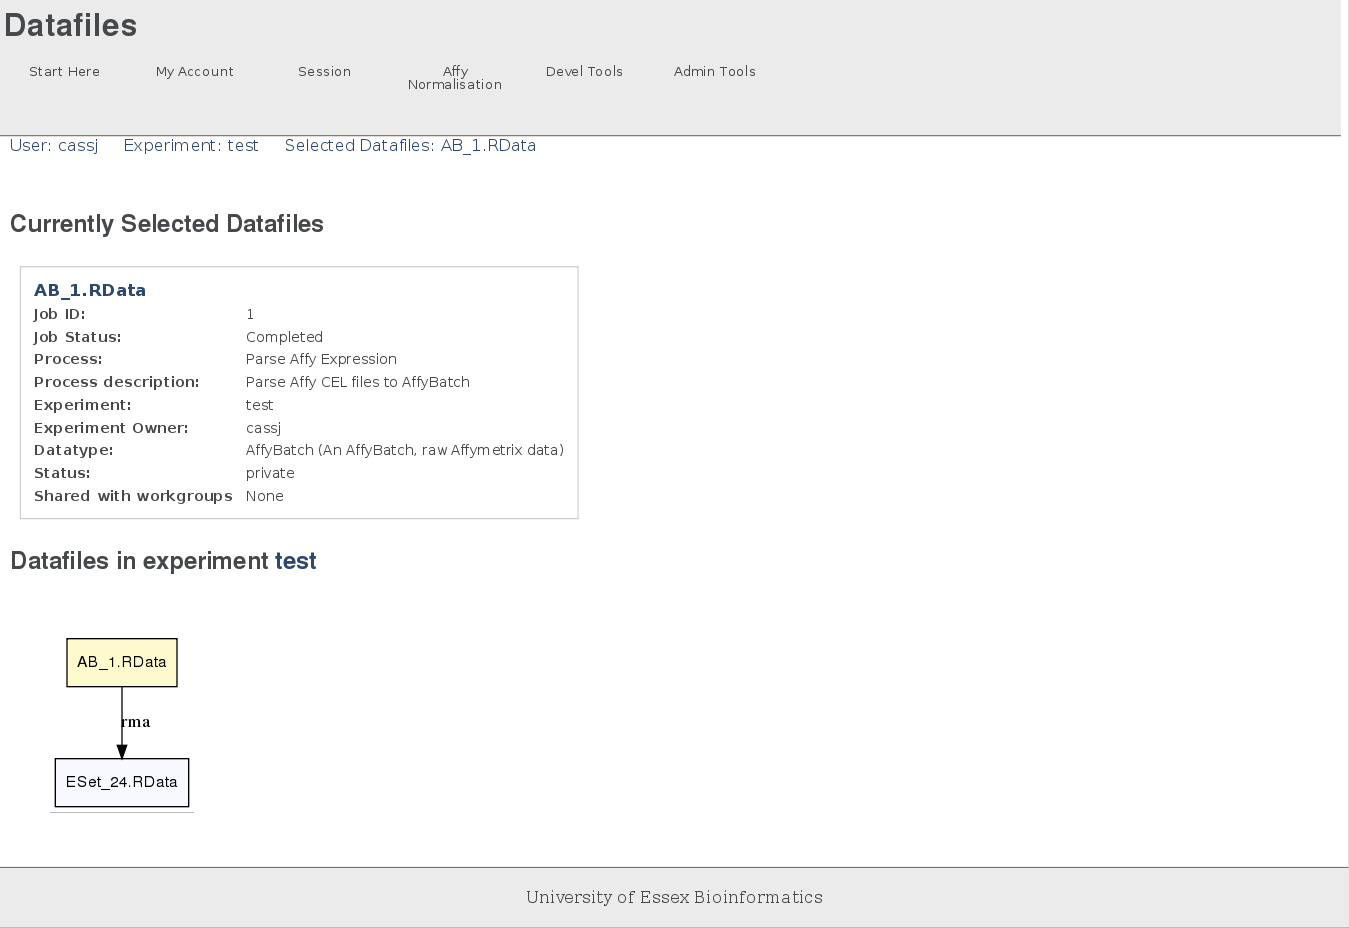
\includegraphics[scale=1]{images/datafiles}
% \caption{Datafiles - I need to do a new image here. ignore this one}\label{fig:datafiles}
% \end{figure}
% 
% %\paragraph*{}
% % They may only accept a single datafile, though this file may be one of a number of acceptable types. In other words, a datafile can only ever have a single parent (see \ref{fig:datafiles}). This does not mean that a component only has access to a single datafile, merely that if it wants to find other related datafiles it should start at the one it has and traverse the tree. This is simply to ensure that the files are actually related in the manner in which the component requires. 
% 
% \paragraph*{Report and Image files}
% Components can also generate \verb|Report Files| and \verb|Image Files|. These are both exported file types that should be served statically for the user to download. Examples include tab-delimited text file exports of data or quality control plots. These file types both have a datafile parent but they are stored in seperate database tables as they require additional information, such as dimensions or filetype.
%   
% \paragraph*{Composite report files}
% The final possible result of a process is a composite report file. This allows you to combine multiple report and image files into a single report file. These files have a seperate table in the database with information about their structure, contents and filetype.
% 
% 
% 
% 
